% latex table generated in R 2.15.3 by xtable 1.7-1 package
% Mon Apr 28 15:44:09 2014
\begin{table*}[ht]
\centering
\begin{tabular}{rp{16em}rrrrc}
  \hline
Feature & Description & quant\_5 & mean & median & quant\_95 & histogram \\ 
  \hline
loc & Lines of code. & 267.00 & 16211.15 & 4878.00 & 61719.60 & 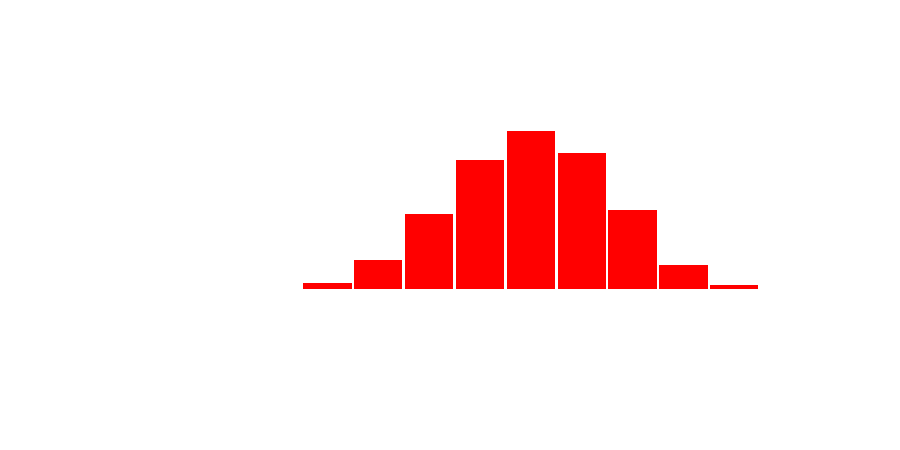
\includegraphics[scale = 0.1, clip = true, trim= 50px 60px 50px 60px]{hist-4fea7249a109b9e1d6791b4c1ebc1f38.pdf} \\ 
  ehloc & Lines of code devoted to exception handling. & 1.00 & 753.12 & 167.00 & 2759.00 & 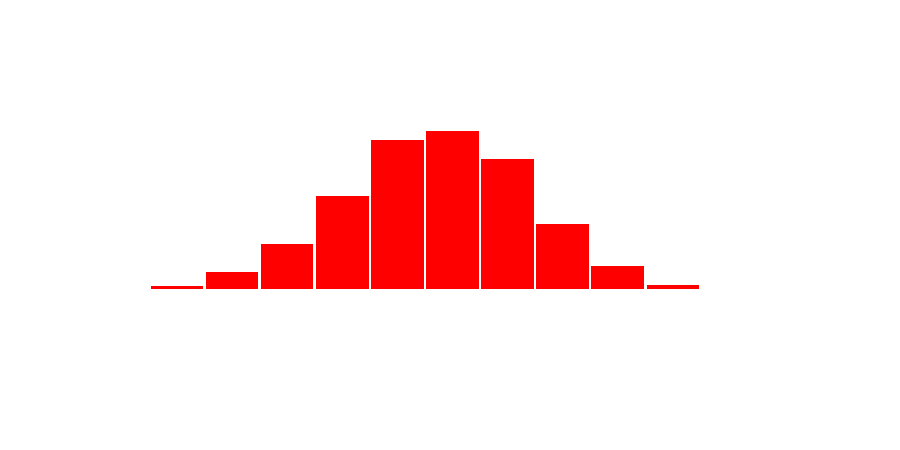
\includegraphics[scale = 0.1, clip = true, trim= 50px 60px 50px 60px]{hist-40db73293da278b6983709bc45b14f55.pdf} \\ 
  num\_classes & Number of user defined exception types. & 3.00 & 173.95 & 59.00 & 681.60 & 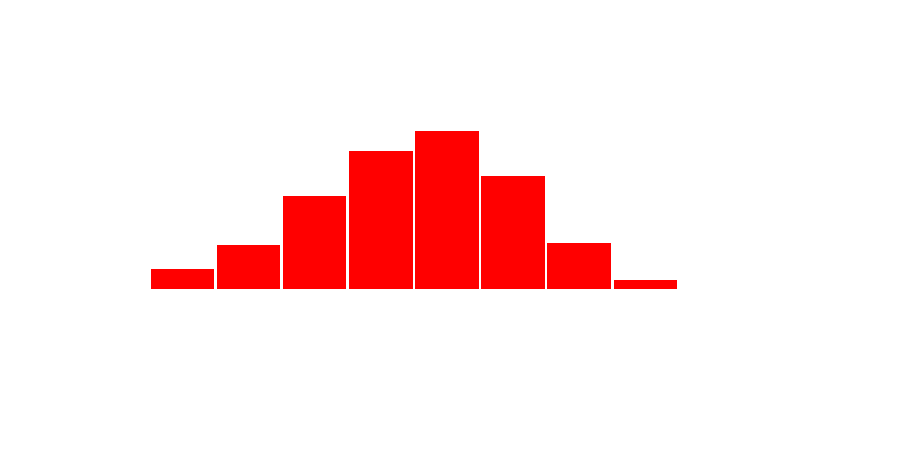
\includegraphics[scale = 0.1, clip = true, trim= 50px 60px 50px 60px]{hist-027fd281b3f6bc7386445836eee5d87e.pdf} \\ 
  userdefined\_exceptions & Number of classes. & 0.00 & 3.09 & 0.00 & 14.00 & 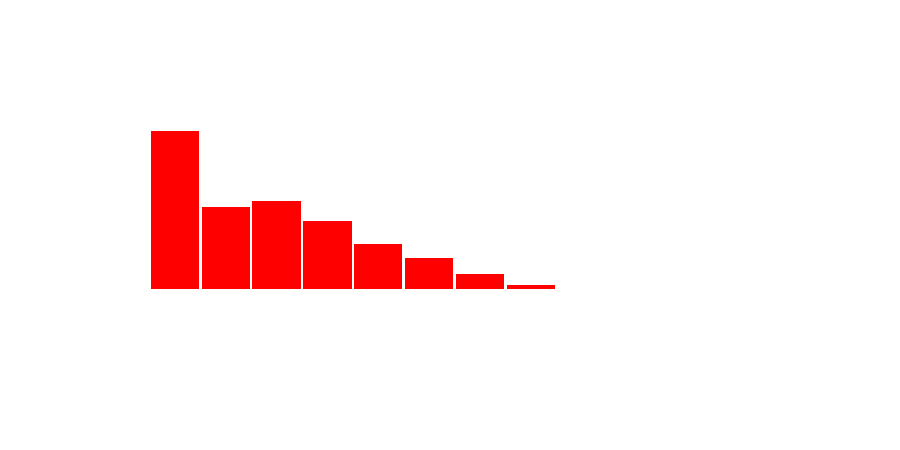
\includegraphics[scale = 0.1, clip = true, trim= 50px 60px 50px 60px]{hist-135e03395e7521809f10de2e03c70b19.pdf} \\ 
  num\_methods & Number of methods. & 12.00 & 1220.10 & 364.00 & 4564.00 & 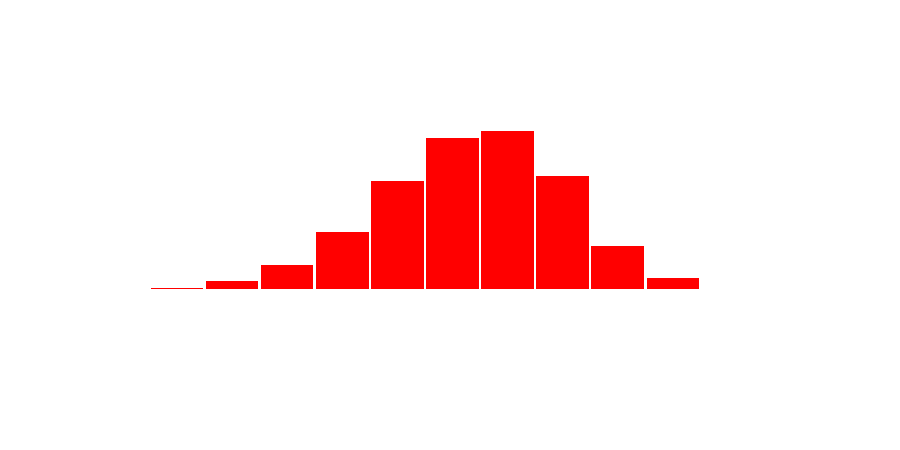
\includegraphics[scale = 0.1, clip = true, trim= 50px 60px 50px 60px]{hist-b6b0d4aa4024bfd6f76543e50b59b4a4.pdf} \\ 
  num\_methods\_throw & Number of methods that throw an exception. & 0.00 & 161.19 & 26.00 & 679.20 & 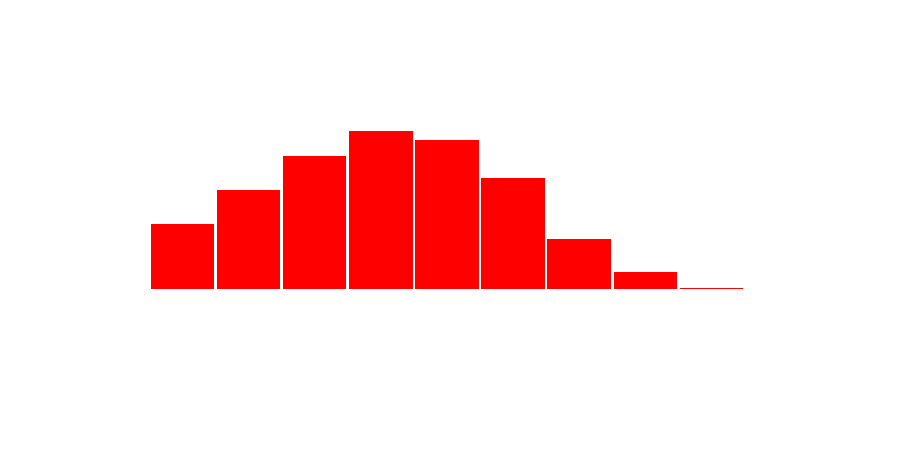
\includegraphics[scale = 0.1, clip = true, trim= 50px 60px 50px 60px]{hist-762ba48e13fc4bdec8910cf5d8e488c1.pdf} \\ 
  num\_public\_methods & Number of public methods. & 8.00 & 907.93 & 260.00 & 3578.20 & 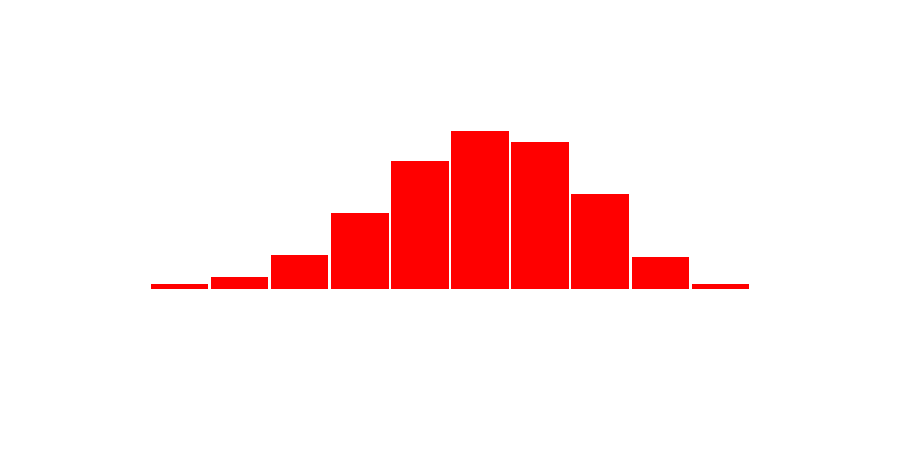
\includegraphics[scale = 0.1, clip = true, trim= 50px 60px 50px 60px]{hist-6a589f87539a5232bab5b7cb76849876.pdf} \\ 
  num\_public\_methods\_throws & Number of public methods that throw an exception. & 0.00 & 114.16 & 16.00 & 507.80 & 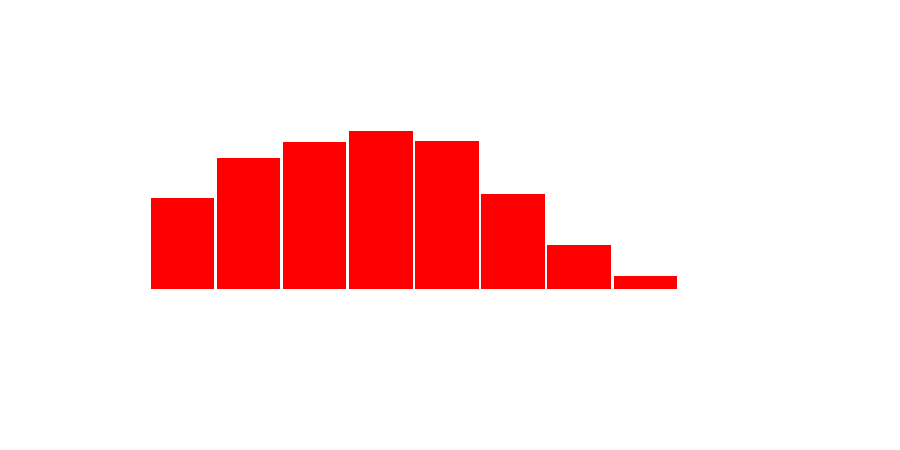
\includegraphics[scale = 0.1, clip = true, trim= 50px 60px 50px 60px]{hist-abd19a466fed24b2e5ab69fd7b2523df.pdf} \\ 
  num\_nonpublic\_methods & Number of private/protected/package methods. & 3.00 & 312.17 & 85.00 & 1281.60 & 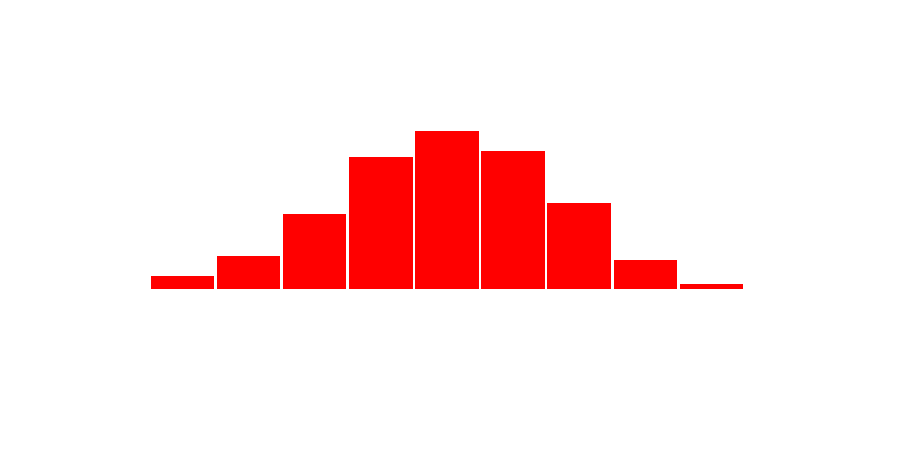
\includegraphics[scale = 0.1, clip = true, trim= 50px 60px 50px 60px]{hist-5ffac6360ae85e10530d281920f084d5.pdf} \\ 
  num\_nonpublic\_methods\_throws & Number of private/protected/package methods that throw an exception. & 0.00 & 47.02 & 7.00 & 169.00 & 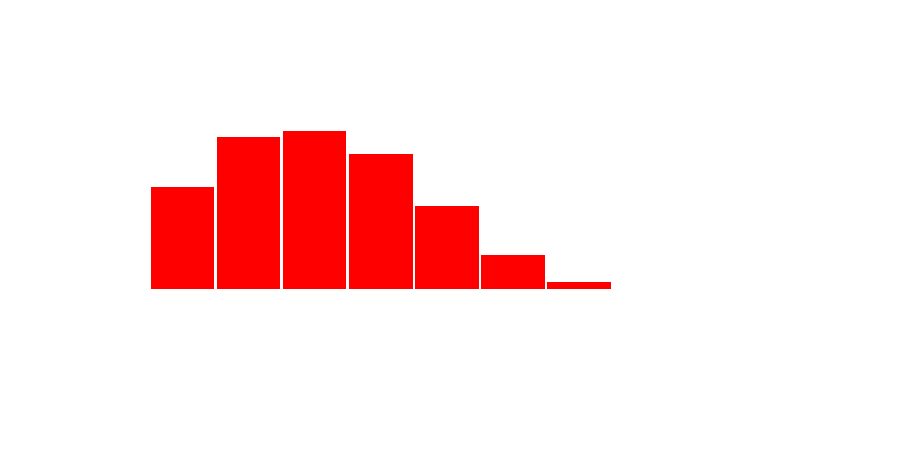
\includegraphics[scale = 0.1, clip = true, trim= 50px 60px 50px 60px]{hist-3ed6823532ea8acc01d29f33cf9379a8.pdf} \\ 
  num\_throw\_statements & Number of throw statements. & 0.00 & 109.38 & 18.00 & 437.60 & 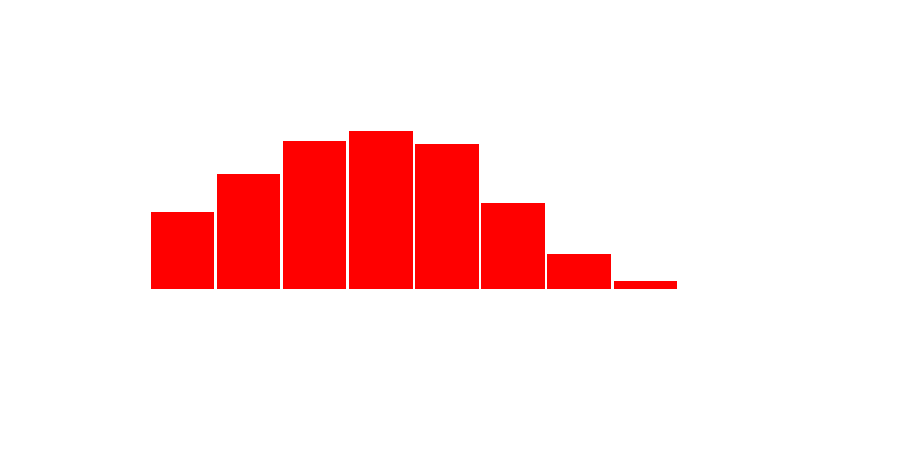
\includegraphics[scale = 0.1, clip = true, trim= 50px 60px 50px 60px]{hist-b25888a559b579f477c029e39bd403d8.pdf} \\ 
  num\_try & Number of try blocks. & 0.00 & 119.08 & 30.00 & 446.00 & 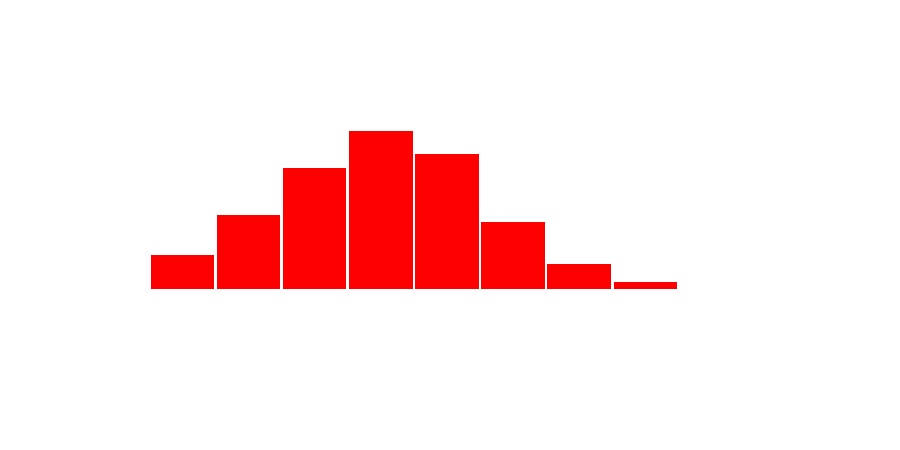
\includegraphics[scale = 0.1, clip = true, trim= 50px 60px 50px 60px]{hist-37304fd9b59fe8289145f1008ad89ad9.pdf} \\ 
  num\_catch & Number of catch blocks. & 0.00 & 119.32 & 32.00 & 451.30 & 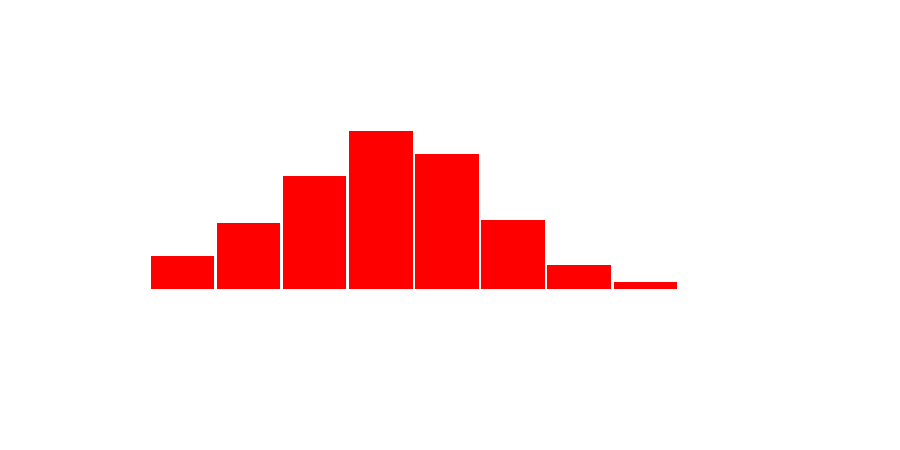
\includegraphics[scale = 0.1, clip = true, trim= 50px 60px 50px 60px]{hist-afc847f0b6862e86823253de78fc0d16.pdf} \\ 
  throw\_on\_catch & Number of try blocks that throw an exception. & 0.00 & 29.24 & 4.00 & 127.00 & 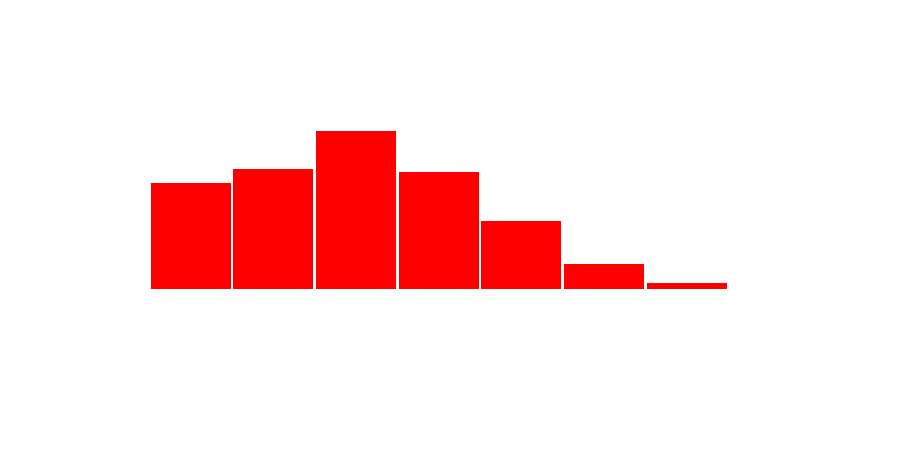
\includegraphics[scale = 0.1, clip = true, trim= 50px 60px 50px 60px]{hist-98dd667c113add4bb8ccce60ef1cb8d7.pdf} \\ 
  return\_on\_catch & Number of catch blocks with an explicit return statement. & 0.00 & 11.91 & 2.00 & 50.00 & 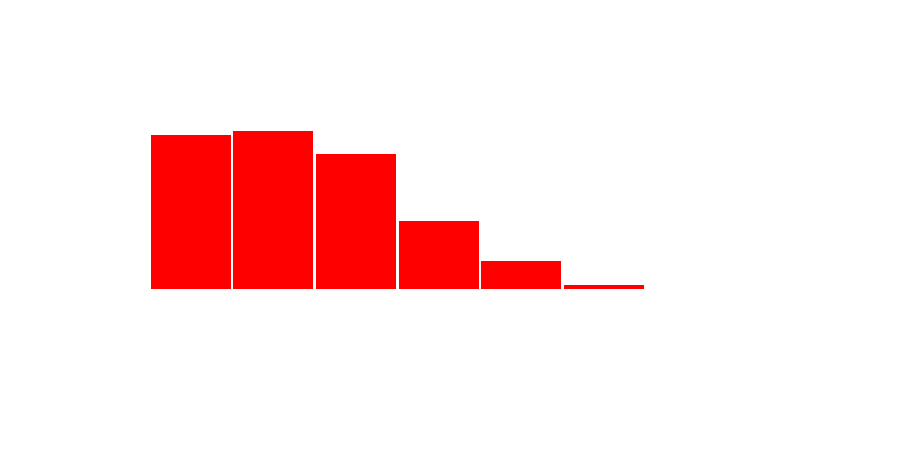
\includegraphics[scale = 0.1, clip = true, trim= 50px 60px 50px 60px]{hist-f9a7775b7b8e5425ef21fcd168e80196.pdf} \\ 
  return\_on\_finall & Number of finally blocks with an explicit return statement. & 0.00 & 0.44 & 0.00 & 0.00 & 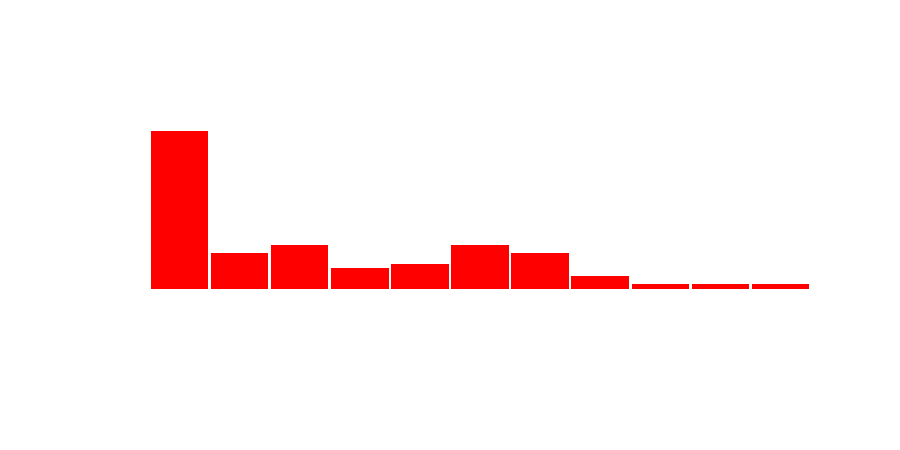
\includegraphics[scale = 0.1, clip = true, trim= 50px 60px 50px 60px]{hist-5b9c377bd3fc66fbdbd3e345bf1f1665.pdf} \\ 
  log\_on\_finally & Number of finally blocks including logging statements. & 0.00 & 0.76 & 0.00 & 3.00 & 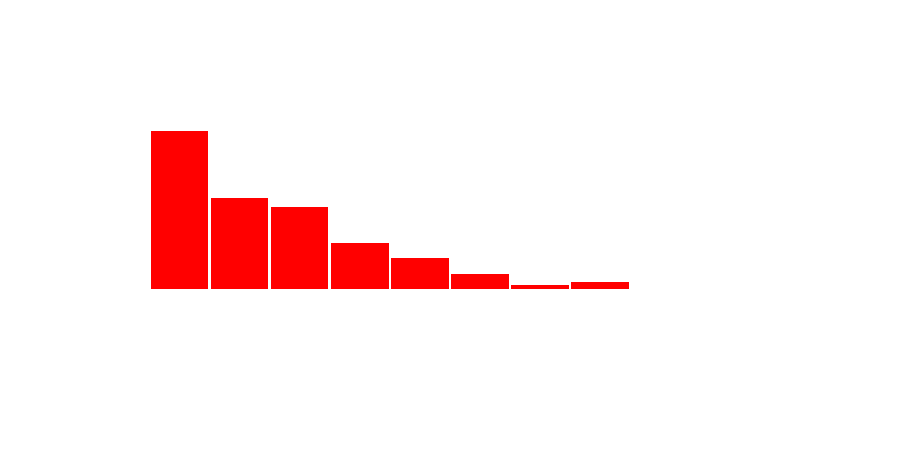
\includegraphics[scale = 0.1, clip = true, trim= 50px 60px 50px 60px]{hist-5f1e0aa338cc8aba188c8b993766730e.pdf} \\ 
  specific\_action\_onfinally & Number of finally blocks including resource cleanup actions. & 0.00 & 28.81 & 0.00 & 84.00 & 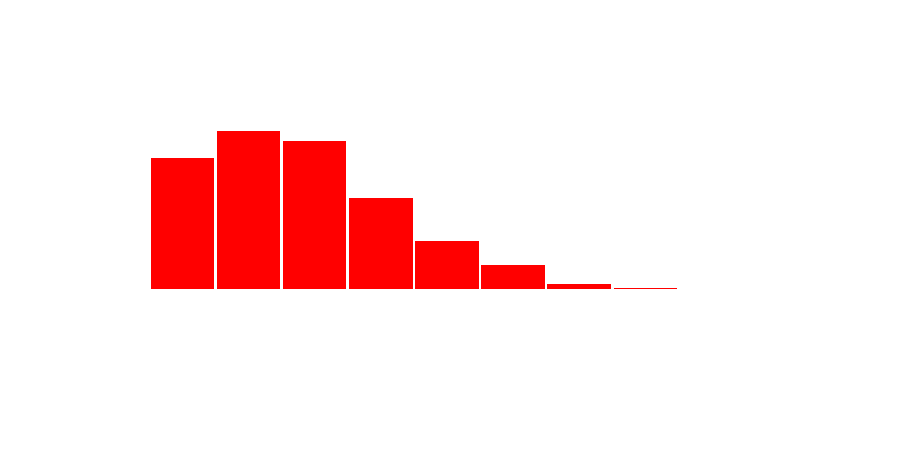
\includegraphics[scale = 0.1, clip = true, trim= 50px 60px 50px 60px]{hist-b7598a0e0c1a6992089680d29db9c202.pdf} \\ 
   \hline
\end{tabular}
\caption{Descriptive statistics for the Java dataset. Historgrams are in log scale.} 
\label{tab:java-descr-stats}
\end{table*}
